Jako první určíme rozměry tranzistoru zrcadla.
Volím délku kanálu \(L = 2 [\mu m]\) jako kompromis mezi velikostí a parametrem \(\lambda\) která pro \(L = 2 \mu m\) nabívá hodnoty \(\lambda = 0.0441692 [V^{-1}]\).
Dále musíme zvolit napětí \(U_{OV}\) které volím s ohledem na rozsah napájecího napětí \(U_{OV} = 0.2 [V]\)
Z toho následně můžeme určit šířku kanálu \(W\), tranzistorů \(M1\) jako:

\begin{center}
    \large
    \(
        W_{M1} = L \cdot \frac{2 \cdot I_1}{KP \cdot U_{OV}^2} = 2\mu \cdot \frac{2 \cdot 10\mu}{200\mu 0.2^2} = 5 [\mu m]
    \)
\end{center}

Z Toho snadno určíme \(W_{M4}\) a \(W_{5}\) jako:

\begin{center}
    \large
    \(
        W_{M2} = W_{M3} = W_{M1} \cdot \frac{I_2}{I_1} = 5\mu \cdot \frac{20\mu}{10\mu} = 10 [\mu m]
    \)
\end{center}

Při určování hodnoty odporu nastavujícího proud \(I_1\) musíme vzít v potas bulk efekt tranzistoru  a určíme jako:

\begin{center}
    \large
    \(
        R = \frac{V_{CC} - (U_{TH-M2} + U_{OV-M2} + U_{TH-M3} + U_{OV-M3})}{I_1} = \frac{1.8 - (0.384 + 0.2 + 0.541 + 2)}{10\mu} = 47.4 [k\Omega] 
    \)
\end{center}

Výstupní rozsah můžeme určit jako:
\begin{center}
    \large
    \(
        U_{out} = U_{CC} - (U_{TH-M2} + U_{OV-M2} + U_{OV-M3}) = 1.8 - (0.363+0.2+0.2) = 1.037 [V]
    \)
\end{center}

Následně můžeme určit výstupní odpor jako:
\begin{center}
    \Large
    \(
        R_{out} = r_{ds3} \left[ 1 + g_{m1} \cdot \frac{r_{ds1} \cdot R}{r_{ds1} + R} \right] = \frac{1}{\lambda \cdot I_2} \left[ 1 + g_{m1} \cdot \frac{\frac{1}{\lambda \cdot I_1} \cdot R}{\frac{1}{\lambda \cdot I_1} + R} \right]
    \)
    \(
        R_{out} = \frac{1}{0.0441692 \cdot 20\mu} \cdot \left[ 1 +  140.8\mu \cdot \frac{\frac{1}{0.0441692 \cdot 10\mu} \cdot 47.4k}{\frac{1}{0.0441692 \cdot 10\mu} + 47.4k}\right] = 8.532 [M\Omega]
    \)
\end{center}

\begin{figure}[h!]
    \centering
    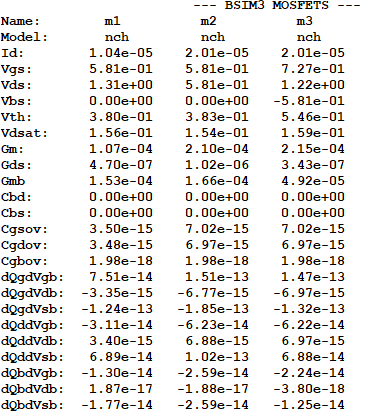
\includegraphics[width=0.6\textwidth]{text/img/WPZ-op-OL.png}
    \caption{\label{fig:WPZ-op-OL} Pracovní body jednotlivých tranzistorů}
\end{figure}

\begin{figure}[h!]
    \centering
    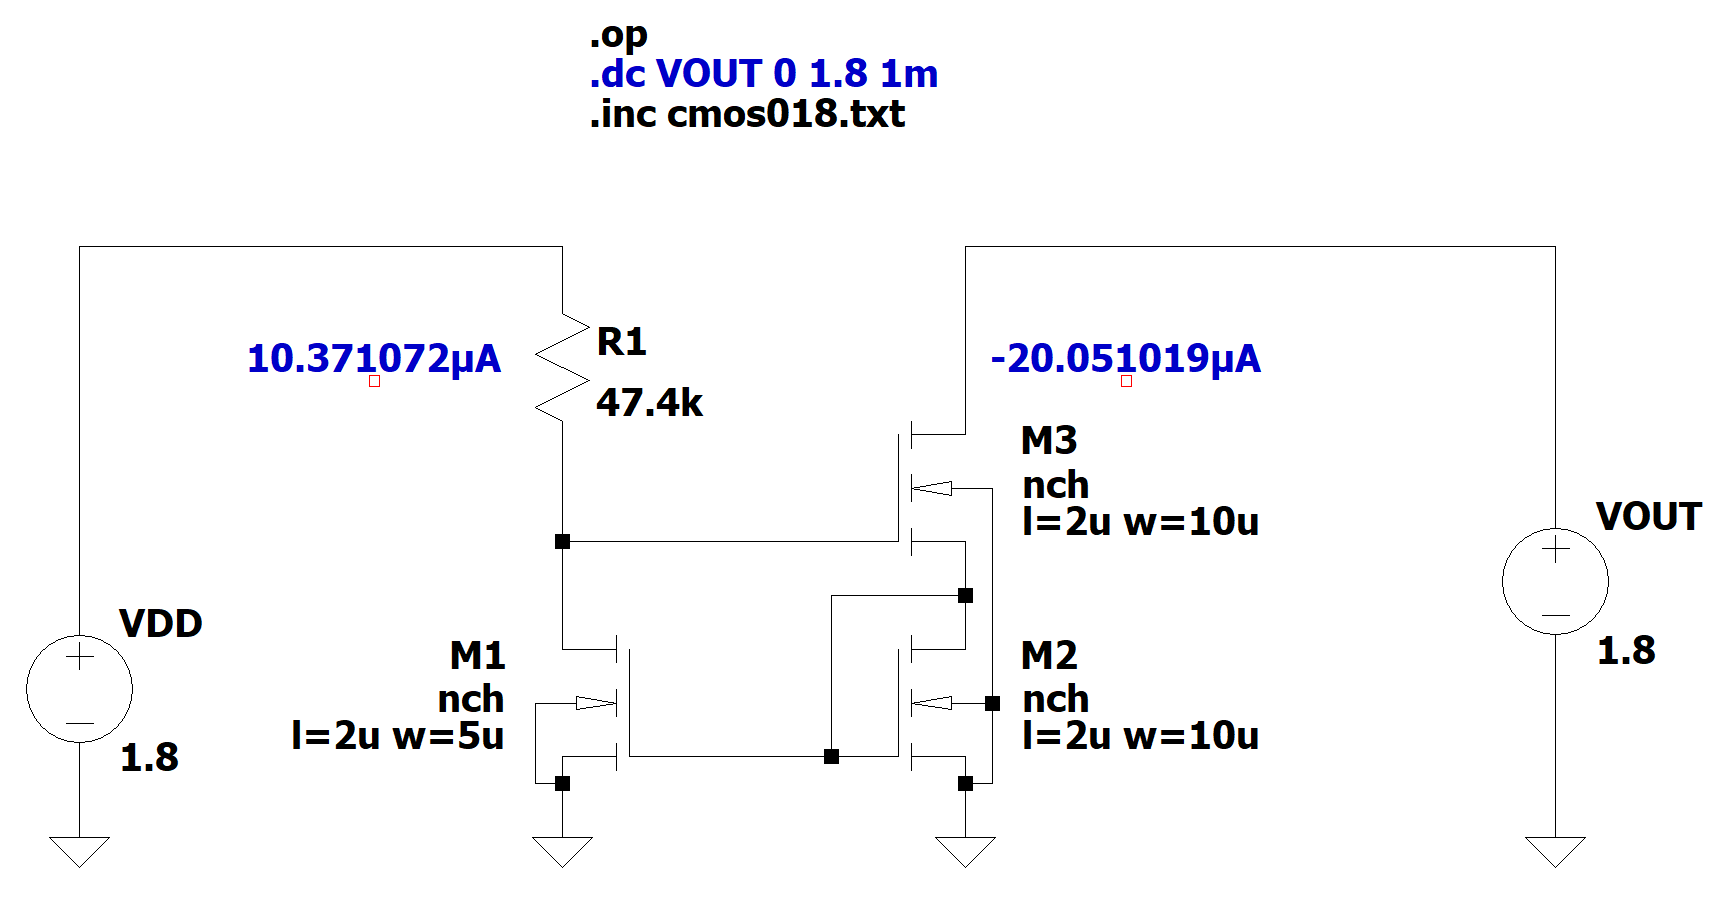
\includegraphics[width=0.9\textwidth]{text/img/WPZ-op-sch.png}
    \caption{\label{fig:WPZ-op-sch} Výsledné schéma s vyznačenými proudy \(I_1\) a \(I_2\)}
\end{figure}

\begin{figure}[h!]
    \centering
    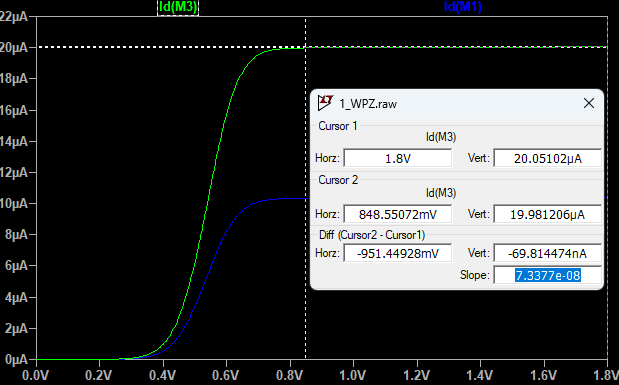
\includegraphics[width=0.9\textwidth]{text/img/WPZ-dc-graf.png}
    \caption{\label{fig:WPZ-dc-graf} Závislost vstupního a výstupního proudu na výstupním napětí}
\end{figure}

Ze simulace můžeme určit výstupní odpor jako:
\begin{center}
    \large
    \(
        r_{out} = \frac{\Delta U}{\Delta I} = \frac{951.4m}{69.814474n} = 14.285 [M\Omega] 
    \)
\end{center}

Což jé téměř dvojnásobek oproti výpočtu, výstupní rozsah naproti tomu sedí poměrně přesně.